\documentclass{article}
\usepackage[margin=0.8in]{geometry}
\usepackage{amsmath}
\usepackage{amssymb}
\usepackage{bookmark}
\usepackage{hyperref}
\usepackage{graphicx}
\usepackage{float}
\usepackage{listings}

\title{Mini-Assignment 2: CS3423 - Compilers - II}
\author{S Vishwak\\
\texttt{CS15BTECH11043}}
\date{}

\begin{document}
\maketitle

\section{Architecture and Design of Polly}
\begin{flushleft}
Polly is a tool used to optimize loops better than those achieved by the regular optimization tags such as \texttt{-O3} or \texttt{-O2}. It operates on the intermediate representation generated by LLVM. Below is a general representation of the compilation of a program using LLVM tools:
\begin{center}
\boxed{\text{Code}} \(\Rightarrow\) \boxed{\text{Tokens}} \(\Rightarrow\) \boxed{\text{AST}} \(\Rightarrow\) \boxed{\text{LLVM IR}} \(\Rightarrow\) \boxed{\text{Optimized LLVM IR}} \(\Rightarrow\) \boxed{\text{Binary}}
\end{center}

Since the focus of this assignment is the optimization w.r.t. Polly, the rest of this section will discuss about the placement and role of Polly in the penultimate step involving raw LLVM IR and the optimized LLVM IR.
\(\newline\)

According to \href{http://polly.llvm.org/docs/Architecture.html}{Polly's Architecture}, every optimization pass i.e., whenever you give the optimization flag (for example: \texttt{-O1}, \texttt{-O2}), there are a series of passes that take place one after the other, which all after completion render the optimized LLVM IR. These phases are broadly listed as follows:
\begin{itemize}
\item Canonicalization
\item Inliner-Cycle
\item Target Specialization
\end{itemize}

\underline{Canonicalization} tries to achieve maximum reduction/elimination of the raw IR using scalar optimizations, hence the name ``canonical". \underline{Inliner-Cycle} focuses on further scalar optimization without disrupting the semantic meaning of the code given and repeatedly tries to inline functions and runs canonicalization passes when the chance of simplification arises, making this a ``Soup algorithm"\footnote{Reference to Ramakrishna sir's notion of Soup algorithm} of sorts. One highlight of the \underline{Inliner-Cycle} is that, simple trivial loop optimizations are done - one such being LICM\footnote{Loop Invariant Code Motion}. Finally comes the \underline{Target Specialization}, which is exactly as it seems - takes into consideration the nature of the target such as the architecture. Some loop transformations occur here.
\(\newline\)

\subsection*{Where does Polly fit in?}
From the looks of it, you could add Polly in two places: 
\begin{itemize}
\item between \underline{Canonicalization} and \underline{Inliner-Cycle}, or
\item between \underline{Inliner-Cycle} and \underline{Target Specialization}
\end{itemize}

This positioning can be controlled using the option \texttt{-polly-position}. The tags taken by this option are: \texttt{early} and \texttt{before-vectorizer}. \texttt{early} indicates placing Polly in the first location suggested and \texttt{before-vectorizer} indicates placing Polly in the second location suggested. There is still some work being performed w.r.t. placing Polly in the second location, hence the default location is \texttt{-polly-position=early}.

\subsection*{How does the location matter?}
When placed in the first location, the optimized code generated by Polly is very similar to the raw LLVM IR. This leads to better understanding of the code produced and consequently better feedback. 
\(\newline\)

When placed in the second location, the Inliner-Cycle has been completed, which means there could be benefits theoretically from running Polly at this location. Since the loop kernel detection time is less, the compile time is not affected greatly. But since LLVM itself performs a whole lot of optimizations in the phases before reaching Polly, practically there could lesser effects than expected.

\subsection*{Capabilities of Polly}
\begin{itemize}
\item Extremely fast loop kernel detection
\item Performs loop optimization on functions which are ``worth" optimizing
\item Low compile time overheads
\end{itemize}
\end{flushleft}

\section{Some experiments with Polly}
\begin{flushleft}
Making some minor modifications to the \texttt{matmul.c}\footnote{Code taken from \texttt{https://github.com/llvm-mirror/polly/blob/master/www/experiments/matmul/matmul.c}} code provided as an example, I ran tests for varying N with 9 options:
\begin{enumerate}
\item Optimization with \texttt{-O3}
\item Optimization with Polly using \texttt{-mllvm -polly}
\item Optimization with Polly and parallelizing using \texttt{-mllvm -polly -mllvm -polly-parallel -llvm -polly-num-threads=i -lgomp} for \texttt{i} ranging from 1 to 4
\item Optimization with Polly using tiling \texttt{-mllvm -polly -mllvm -polly-tiling}
\item Optimization with Polly using vectorization \texttt{-mllvm -polly -mllvm -polly-vectorizer=stripmine}
\item Optimization using both tiling and vectorization
\end{enumerate}

Below are the compile time and run time results obtained:
\begin{figure}[H]
\begin{minipage}{0.45\linewidth}
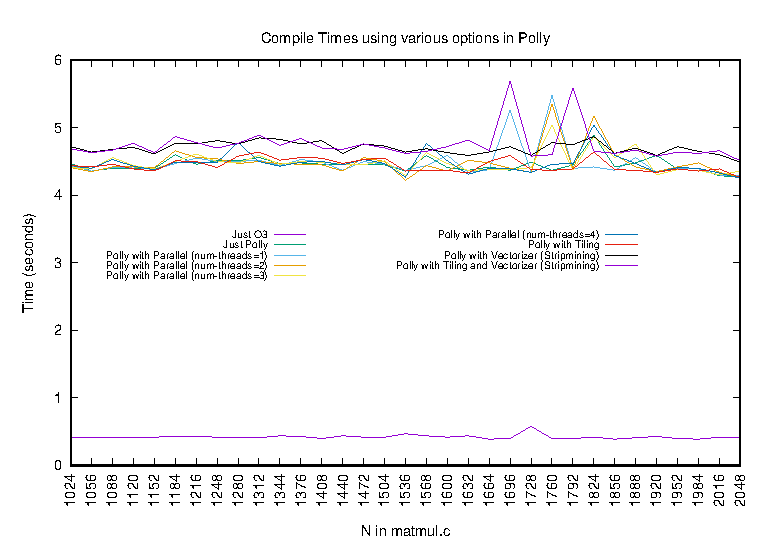
\includegraphics[width=0.9\textwidth]{./images/compile_time.eps}
\caption{Compile Time graph}
\end{minipage}
\hfill
\begin{minipage}{0.45\linewidth}
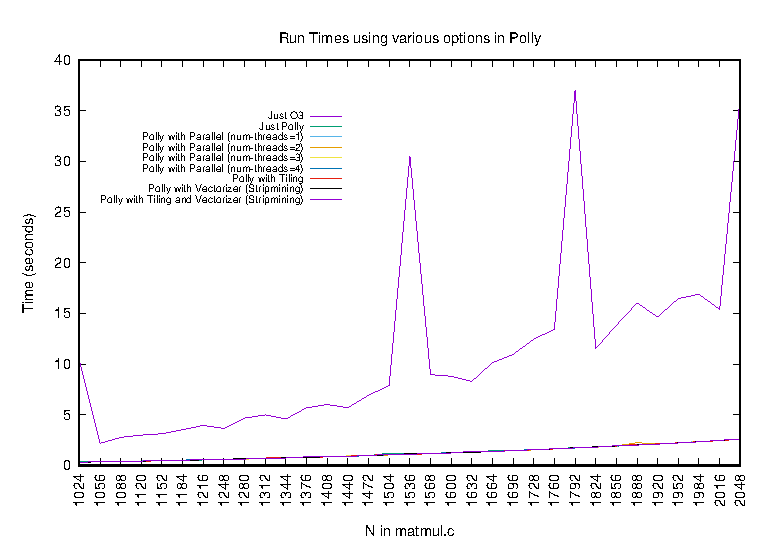
\includegraphics[width=0.9\textwidth]{./images/run_time.eps}
\caption{Run Time graph}
\end{minipage}
\end{figure}

Notice the amazing improvement in the run time over slight increase in compile time for Polly based optimizations.
\end{flushleft}

\section{SCoP and Dependences}
\subsection*{What are SCoPs?}
\begin{flushleft}
A Static Control Part is a set of statements executed consecutively given a set of loop bounds and conditions. These loop bounds and conditionals have to be an affine function of the loop parameters. Also it must be made sure that this set is maximal w.r.t. cardinality i.e., the number of statements has to be as high as possible.
\(\newline\)

Consider an example piece of code:
\begin{lstlisting}
for(int i = 0;i < 10;i++)
{
	for(int j = 0;j < 10;j++)
	{
		foo(i, j);
	}
}
\end{lstlisting}

The SCoP of the above section of code is: \(\{\texttt{stmt} | \texttt{stmt = foo(i, j)} \ni \texttt{ i, j} \in [0, 9] \text{ and } \texttt{i, j} \in \mathbb{Z}\}\). Note that this is maximal: \texttt{foo(i, j)} is executed for every possible pair of \texttt{i} and \texttt{j}. 

It is also possible to write the constraints in an affine manner\footnote{Using the definition in this paper: \href{http://web.cs.ucla.edu/~pouchet/doc/cc-article.10.pdf}{Benabderrahmane et al}} as follows: 
\begin{equation*}
\begin{pmatrix}
1 & 0 \\ 0 & 1 \\ -1 & 0 \\ 0 & -1
\end{pmatrix}
\begin{pmatrix}
i \\ j
\end{pmatrix} + 
\begin{pmatrix}
0 \\ 0 \\ 9 \\ 9 
\end{pmatrix} \geq 0
\end{equation*}

This set of constraints turn out to represent the polyhedral model. The form of expression of the constraints is the reason why the SCoP detected by Polly have replaced \(<\) \texttt{N} with \(\leq\) \texttt{N - 1}.
\end{flushleft}
\subsection*{What are Dependences?}
\begin{flushleft}
Dependences come into picture when the order of execution is taken into account. We can tell a given statement \texttt{P} is dependent on \texttt{Q} if the execution of \texttt{P} is dependent on the result/execution of \texttt{Q}. Dependences\footnote{Most of the definitions and understanding is influenced by \href{https://en.wikipedia.org/wiki/Loop_dependence_analysis}{this Wikipedia page}} are classified into two types: \textit{data dependence} and \textit{control dependence}. \textit{Data dependencies} highlight the dependences of variables in the code whereas, \textit{Control dependencies} highlight the dependencies caused due to the algorithm itself.
\(\newline\)

There are three basic types of \textit{data dependencies}: \textit{true dependence}, \textit{anti dependence} and \textit{output dependence}. 

\subsubsection*{True Dependence}
\textit{True dependence} occurs when a location in memory is written to before being read from. For example, consider \texttt{P: a = 1729} and \texttt{Q: b = a}. Note that \texttt{Q} is true-dependent on \texttt{P}, otherwise the value of \texttt{b} would be junk. In the context of loops: it could happen that the statement to be executed in the current iteration is dependent on the previous iteration (like recursion). 

\subsubsection*{Anti Dependence}
\textit{Anti dependence} occurs when a location in memory is written to after being read from. Considering the same \texttt{P} and \texttt{Q}, we should be able to see that \texttt{P} is anti dependent on \texttt{Q}, if the order of execution is \texttt{Q}, then \texttt{P}. In the context of loops: it could happen that the statement to be executed reads from a variable and in the next iteration that variable is over-written. 

\subsubsection*{Output Dependence}
\textit{Output dependence} occurs when a location in memory is written to after being written to before. Consider the modified statement \texttt{R: b = 153}. Note that if the execution order is: \(\texttt{P} \rightarrow \texttt{Q} \rightarrow \texttt{R}\), then there is an output dependence between \texttt{Q} and \texttt{R}. In the context of loops: it could happen that there is a conditional counter, which is initialized at the beginning of the iteration, and modified every time the condition is satisfied. Generally all counter-based statements possess output dependence.

\subsubsection*{Control Dependencies}
\textit{Control dependence} occurs when the order of the execution of a set of statements is controlled - possibly by an algorithm. Example is an \texttt{if-then-else} statement, where the \texttt{if} check controls which set of statements are to be executed. 
\end{flushleft}

\section{Analysis of Polly generated IR and normal IR before optimizing}
\end{document}
